\subsubsection{S and B extraction}
To be completed 

\subsubsection{Background correlation shape}
To be completed

\subsubsection{D-meson cut stability}
To be completed

\subsubsection{Tracking efficiency}
To be completed

\subsubsection{DCA cut stability}
To be completed

\subsubsection{Feed-down subtraction}
To be completed

\subsubsection{Correction for bias on B to D decay topologies}
To be completed

\subsubsection{Final table of systematics on correlation distributions}
To be completed

\subsubsection{Uncertainties on fit observables}
The evaluation of the systematic uncertainty on the fit observables is exactly the same as that described in subsection 5.3 for the centrality-integrated analysis (but considering, of course, in each centrality class the corresponding uncertainty values, as described in the previous section).
The only modification involves the values chosen for the $v_2$ hypothesis (also dealt in subsection 5.3), which are differentiated on the bases of the centrality class.
The hypotheses on the charged particle $v_2$ versus centrality were guessed on the bases of the results shown in Fig. \ref{fig:v2h}, taken from the analysis note on charged hadron $v_2$ in p--Pb collisions (2016 sample) in different V0A multiplicity classes. Though the estimator is different from the ZNA we use, the rather flat values of $v_2$ versus centrality ensures the possibility of using these results as reference.

\begin{figure}
\centering
{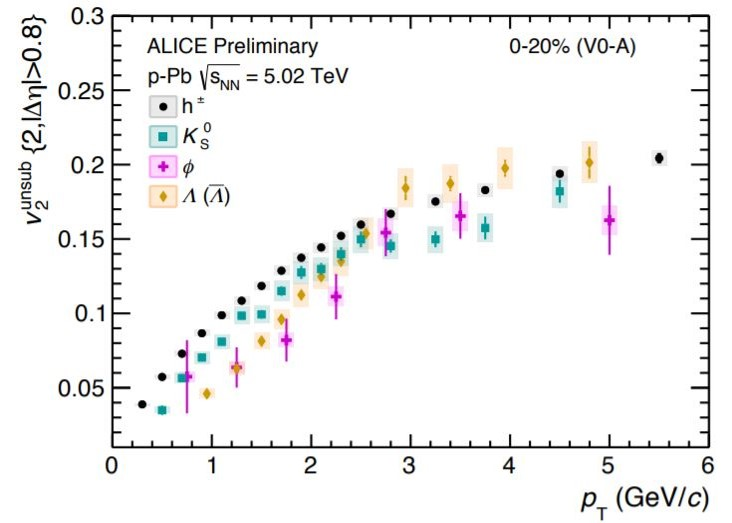
\includegraphics[width=0.45\linewidth]{figuresVsCent/Global/v2/v2h1.jpg}}
{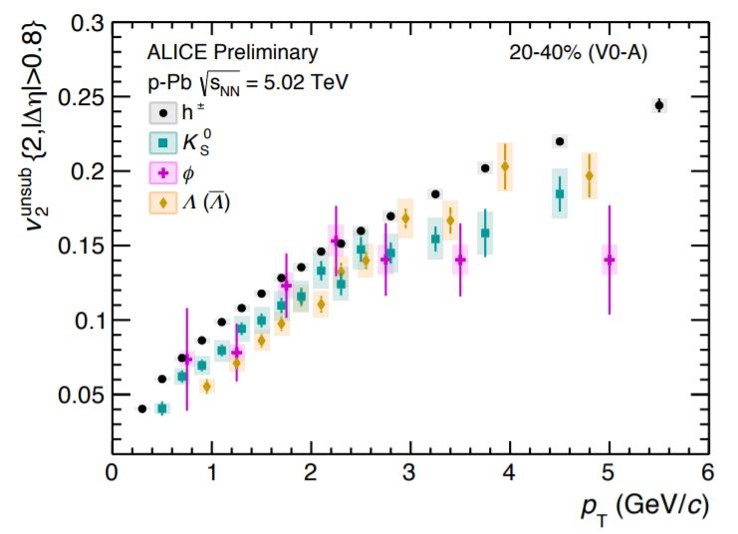
\includegraphics[width=0.45\linewidth]{figuresVsCent/Global/v2/v2h2.jpg}} \\
{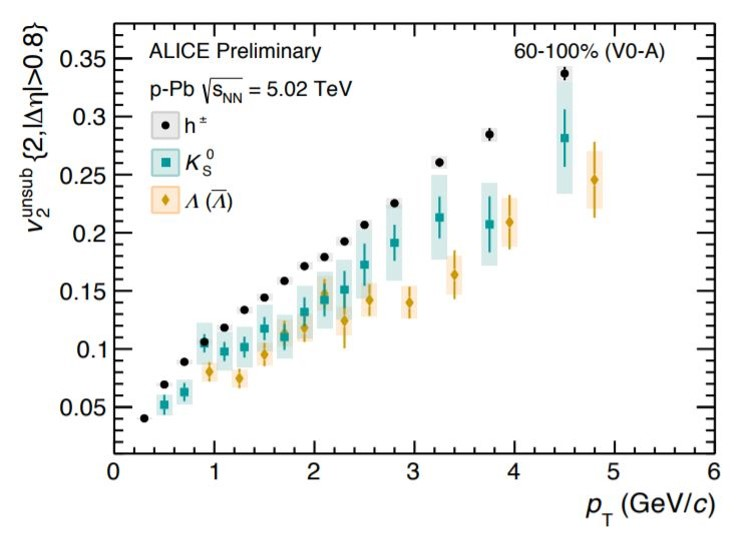
\includegraphics[width=0.45\linewidth]{figuresVsCent/Global/v2/v2h3.jpg}}
 \caption{Reference plots for estimation of $v_2$(h) hypotheses in the three CC.}
\label{fig:v2h}
\end{figure}

The hypotheses on D-meson $v_2$ were guessed starting from ALICE preliminary results of heavy-flavour decay electron $v_2$ in the same collision system, using the ZNA estimator (left panel of \ref{fig:v2D}. The measurement was performed in lower $\pt$(e) ranges, but which by chance are fairly similar to the average $\pt$ of out D-meson correlation ranges, if the $\pt$ of the parent D-hadron is considered for charm-origin heavy-flavour decay electrons - as shown in the right panel of Fig. \ref{fig:v2D}. The drawback of this choice relies in the fact that these $v_2$ values are obtained after the HM-LM subtraction, while in our analysis we need hypotheses for $v_2$ in each CC (considering this, we used just flat values in each CC following the charged particle trend), and also in the fact that heavy-flavour electron $v_2$ includes the contribution from, beauty-hadron decay electrons (though small for $\pt < 3$ GeV/$c$), while the B-feed-down is instead subtracted in our D-meson analysis.

\begin{figure}
\centering
{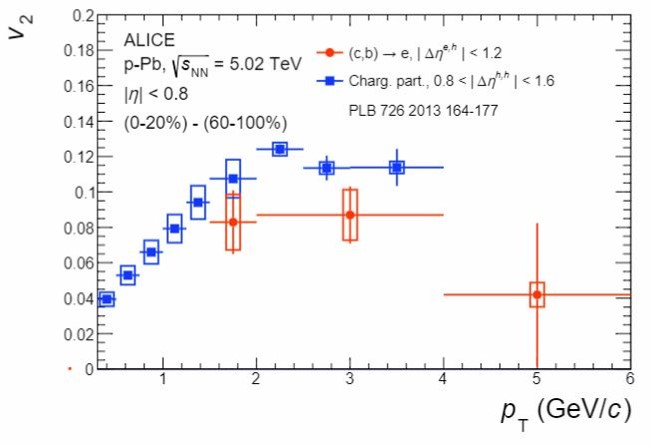
\includegraphics[width=0.4\linewidth]{figuresVsCent/Global/v2/v2D1.jpg}}
{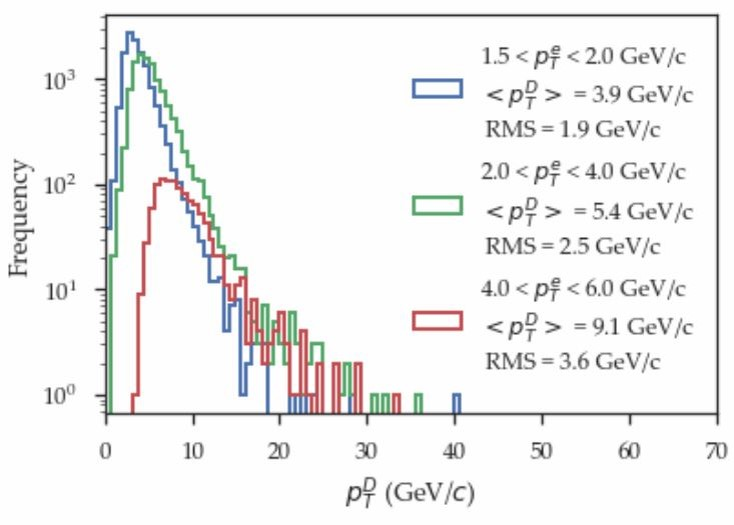
\includegraphics[width=0.4\linewidth]{figuresVsCent/Global/v2/v2D2.jpg}}
 \caption{Left: $v_2$ of heavy-flavour decay electrons in p--Pb, after HM-LM subtraction. Right: corrispondence of $\pt$(e) and $\pt$ of the parent D-meson (for charm-origin electrons).}
\label{fig:v2D}
\end{figure}

In the following, thus, we enlist the $v_2$ hypotheses we adopted for the evaluation of the systematic on the fit observables due to a possible presence of flow:
\begin{itemize}
  \item For 0-20\%: 0.08, 0.08, 0.04, 0.02 (for $\pt$(D) 3-5, 5-8, 8-16, 16-24 GeV/$c$); 0.08, 0.05, 0.11 (for $\pt$(assoc) $>0.3$, 0.3-1, $>1$ GeV/$c$)
  \item For 20-60\%: 0.08, 0.08, 0.04, 0.02 (for $\pt$(D) 3-5, 5-8, 8-16, 16-24 GeV/$c$); 0.08, 0.05, 0.11 (for $\pt$(assoc) $>0.3$, 0.3-1, $>1$ GeV/$c$)
  \item For 60-100\%: 0.08, 0.08, 0.04, 0.02 (for $\pt$(D) 3-5, 5-8, 8-16, 16-24 GeV/$c$); 0.10, 0.06, 0.13 (for $\pt$(assoc) $>0.3$, 0.3-1, $>1$ GeV/$c$)
\end{itemize}
